\section{Data}
\label{sec:data}

Studying firm responses at the threshold needs firm-level turnover near the
cutoff, which the official statistics publish only in coarse turnover bands. I
therefore build a synthetic firm population calibrated to those aggregates: it
reproduces the official totals while resolving the individual firm that the
authorities do not release, opening the analysis to anyone. The same
calibrate-to-published-aggregates approach underlies open household-level
tax-benefit microsimulation \citep{policyengine}; here I apply it at the firm
level. The generator takes the registration threshold as a parameter and is
documented in Appendix~\ref{app:data}; I build one population for 2023--24
(threshold \pounds85{,}000), the paper's primary data year, and one for
2024--25 (threshold \pounds90{,}000), used for the forward sweep of
Section~\ref{sec:static}.

The archived CSV inputs in this repository remain the reproduction source for
the paper's reported numbers; a pinned migration snapshot also represents the
same numeric target surface through PolicyEngine Ledger and the
experimental Populace firm generator, and Appendix~\ref{app:data} reports the
parity check between that shared source-of-truth path and the paper inputs.

\paragraph{Construction.} Index firms by $i$. For each sector $s$ and ONS
turnover band $b=[\underline{b},\overline{b}]$, the \emph{UK Business: Activity,
Size and Location} table gives a business count $N_{s,b}$, and I draw $N_{s,b}$
firms with within-band turnover
\[
  y_i \;=\; \underline{b} + (\overline{b}-\underline{b})\,u_i + \varepsilon_i,
  \qquad u_i \sim \mathcal{U}(0,1), \;\; \varepsilon_i \sim \mathcal{N}(0,\sigma_b^2),
\]
truncated below at zero, where $\varepsilon_i$ smooths the within-band
distribution. The ONS register covers businesses registered for VAT and/or
PAYE---about 2.7 million---so the synthetic population represents that
registered-business frame, not the full business population of roughly
5.6 million in the DBT business population estimates; the difference is
concentrated below the threshold and matters for threshold \emph{cuts}, which I
flag where relevant. Each firm is given input expenditure $x_i = \rho_i\,y_i$,
with the input--output ratio $\rho_i$ drawn from a rescaled Beta distribution
with sector-specific shifts, clamped to $\rho_i \in [0.1, 0.95]$ (mean about
0.6, so value added averages about 40\% of turnover, in line with the UK
non-financial business economy). Its net VAT liability is the standard rate
applied to its value added,
\[
  v_i \;=\; \tau\,(y_i - x_i), \qquad \tau = 0.20,
\]
so every firm's net rate $v_i/y_i = \tau(1-\rho_i)$ lies in $[1\%, 18\%]$,
strictly positive and below the statutory cap of 20\%. The model therefore
abstracts from net-repayment traders (firms with zero-rated outputs whose input
reclaim exceeds output VAT---HMRC's negative-liability column); representing
them requires rated-structure detail (zero, reduced, and exempt output shares)
that the public aggregates do not resolve by band. Employment is assigned from
the ONS employment-band shares.\footnote{An earlier draft of this generator set
$v_i = y_i - x_i$ with $\rho_i \in [0.6, 1.5]$---omitting the factor $\tau$, so
per-firm liabilities were about five times too large and a large minority of
firms carried negative value added. The weight optimiser compensated on the
band totals, leaving aggregate calibration scores similar but distorting the
near-threshold density; Section~\ref{sec:bunching} documents the consequence
and the correction.}

The base population reproduces the ONS structure but not
the HMRC VAT-registered totals, so I re-weight it. Each firm receives a strictly
positive weight $w_i = e^{\theta_i}$, and for a vector of official targets
$T=(T_k)_{k=1}^{K}$ the weighted synthetic counterpart of target $k$ is
\[
  \widehat{T}_k(\theta) \;=\; \sum_i a_{ki}\, w_i ,
\]
where $a_{ki}$ is firm $i$'s contribution to target $k$: an indicator of band or
sector membership for a count target, and the firm's net liability $v_i$ for a
VAT-liability target. I choose $\theta$ to minimise a symmetric relative-error
loss with per-target importance weights $\lambda_k$,
\[
  L(\theta) \;=\; \frac{1}{K}\sum_{k} \lambda_k
    \min\!\Big\{ \big(\widehat{T}_k/T_k - 1\big)^2,\; \big(T_k/\widehat{T}_k - 1\big)^2 \Big\}
    \;+\; \frac{\alpha}{N}\sum_i \lvert \theta_i \rvert ,
\]
the final term a mean absolute penalty on the log-weights. The targets are the
HMRC VAT-registered counts by turnover band and by sector, the HMRC net VAT
liability by turnover band, the ONS employment-band totals, and---for the
2023--24 vintage---the OBR's published near-threshold profile: the March 2023
\emph{Economic and Fiscal Outlook} Chart~C data give HMRC counts of businesses
by \pounds1{,}000 turnover band over \pounds65{,}000--\pounds90{,}000
\citep{obr2023vat}, which I interpolate to the 2023--24 data year between the
2019--20 outturn and the OBR's 2025--26 frozen-threshold projection. The five
bins at or above the threshold enter as direct count targets (every
firm there is VAT-registered, the same universe as the coarse HMRC band they
refine); the twenty bins below the threshold enter as \emph{shape} targets,
normalised over the \pounds65{,}000--\pounds85{,}000 window and scaled to the
synthetic population's own mass there, because the chart counts a narrower
universe than the ONS business frame below the threshold. These fine targets
pin the near-threshold density to the administratively observed bunching
profile---the region that coarse bands alone leave to the weight optimiser
(Section~\ref{sec:bunching}). No fine bands are published for the
\pounds90{,}000 threshold era, so the 2024--25 vintage keeps coarse bands
only. Turnover-band and near-threshold targets carry the largest $\lambda_k$,
followed by VAT liability by band. VAT liability by sector is reported as an
informational diagnostic but excluded from the optimizer, because the
generator draws a common input-share distribution with sector shifts rather
than calibrating the input/output tax structure by sector. The problem is
solved by gradient descent, and the symmetric loss keeps targets of very
different magnitudes on a common scale.

A firm is registered with certainty when its data-year turnover exceeds the
threshold $T^{*}$. This is an approximation to the statutory test, which is a
rolling 12-month test on \emph{taxable} turnover with a roughly two-month
registration lag, a forward-looking 30-day test, and an exception for temporary
breaches (Section~\ref{sec:background}); the model also registers firms whose
turnover is largely exempt, whom the law would not require to register. For a
single-year cross-section calibrated to registered-population totals these
timing and composition wedges are second order for the aggregates, but they are
worth naming: the HMRC band tables classify traders by total declared outputs
(VAT-return Box 6), and the ONS turnover measure is likewise total turnover, so
the running variable throughout is total rather than taxable turnover. Below
the threshold a firm registers voluntarily with probability $r = M / n_{<}$,
where $M$ is the HMRC count of registered firms in the \pounds1--threshold band
and $n_{<}$ is the unweighted number of synthetic below-threshold firm rows.
This sets the expected row-level voluntary-registration rate; I do not treat
below-threshold voluntary registration as a separate weighted calibration
target. The resulting dataset comprises approximately $2.94$~million firm
records per vintage, weighted to represent roughly $2.5$~million registered
businesses. Checked against the official sources along every calibrated
dimension, both vintages attain an overall calibration accuracy of 89.4\%,
with dimension scores ranging from 77.9\% (2023--24 employment bands) and
79.0\% (2024--25 liability by band) to 94.4\%; Appendix~\ref{app:data} reports
the full table. The headline is the mean of five calibrated-dimension scores,
each clipped at zero as $\max\{0,1-\lvert \widehat{T}-T\rvert/\lvert T\rvert\}$;
it excludes the VAT-liability-by-sector diagnostic described above.

\paragraph{The registration threshold in the data.} My primary data year is
2023--24, when the statutory threshold was \pounds85{,}000. The HMRC band
targets step down across the threshold---678{,}350 firms in the
\pounds1--\pounds85{,}000 band against 305{,}320 in
\pounds85{,}000--\pounds150{,}000, or roughly $8{,}000$ against $4{,}700$ firms
per \pounds1{,}000 of band width---and the calibrated population necessarily
inherits that band-average step. The \emph{local} shape within a few thousand
pounds of the threshold is pinned by the OBR near-threshold targets described
above: the calibrated density rises into the threshold (about $13{,}800$ firms
per \pounds1{,}000 in the \pounds84{,}000--\pounds85{,}000 bin), steps down
across it (about $11{,}500$ just above), and declines through the band---the
administratively observed bunching profile \citep{obr2023vat,liuetal2021},
present in the file because it is targeted, not because any synthetic firm
chooses it. In an earlier build without these targets the local shape was an
unpinned optimiser equilibrium (and, under the pre-correction liability scale,
a spurious bunching look-alike); the central data caveat of the paper stands
in all three configurations: no sub-band feature of band-calibrated synthetic
data carries behavioural information beyond what its targets put there
(Section~\ref{sec:bunching} quantifies this with placebo and recovery tests).
Counterfactual policies---including the \pounds85{,}000 to \pounds90{,}000
reform and the forward threshold sweep of Section~\ref{sec:static}---are
evaluated on these firms by re-applying the registration rule to the microdata
for the static costings, holding the empirical turnover distribution fixed. A
behavioural layer that re-prices firms under counterfactual schedules,
conditional on an assumed turnover elasticity, is developed in
Section~\ref{sec:behavioural}.

\begin{figure}[htbp]
\centering
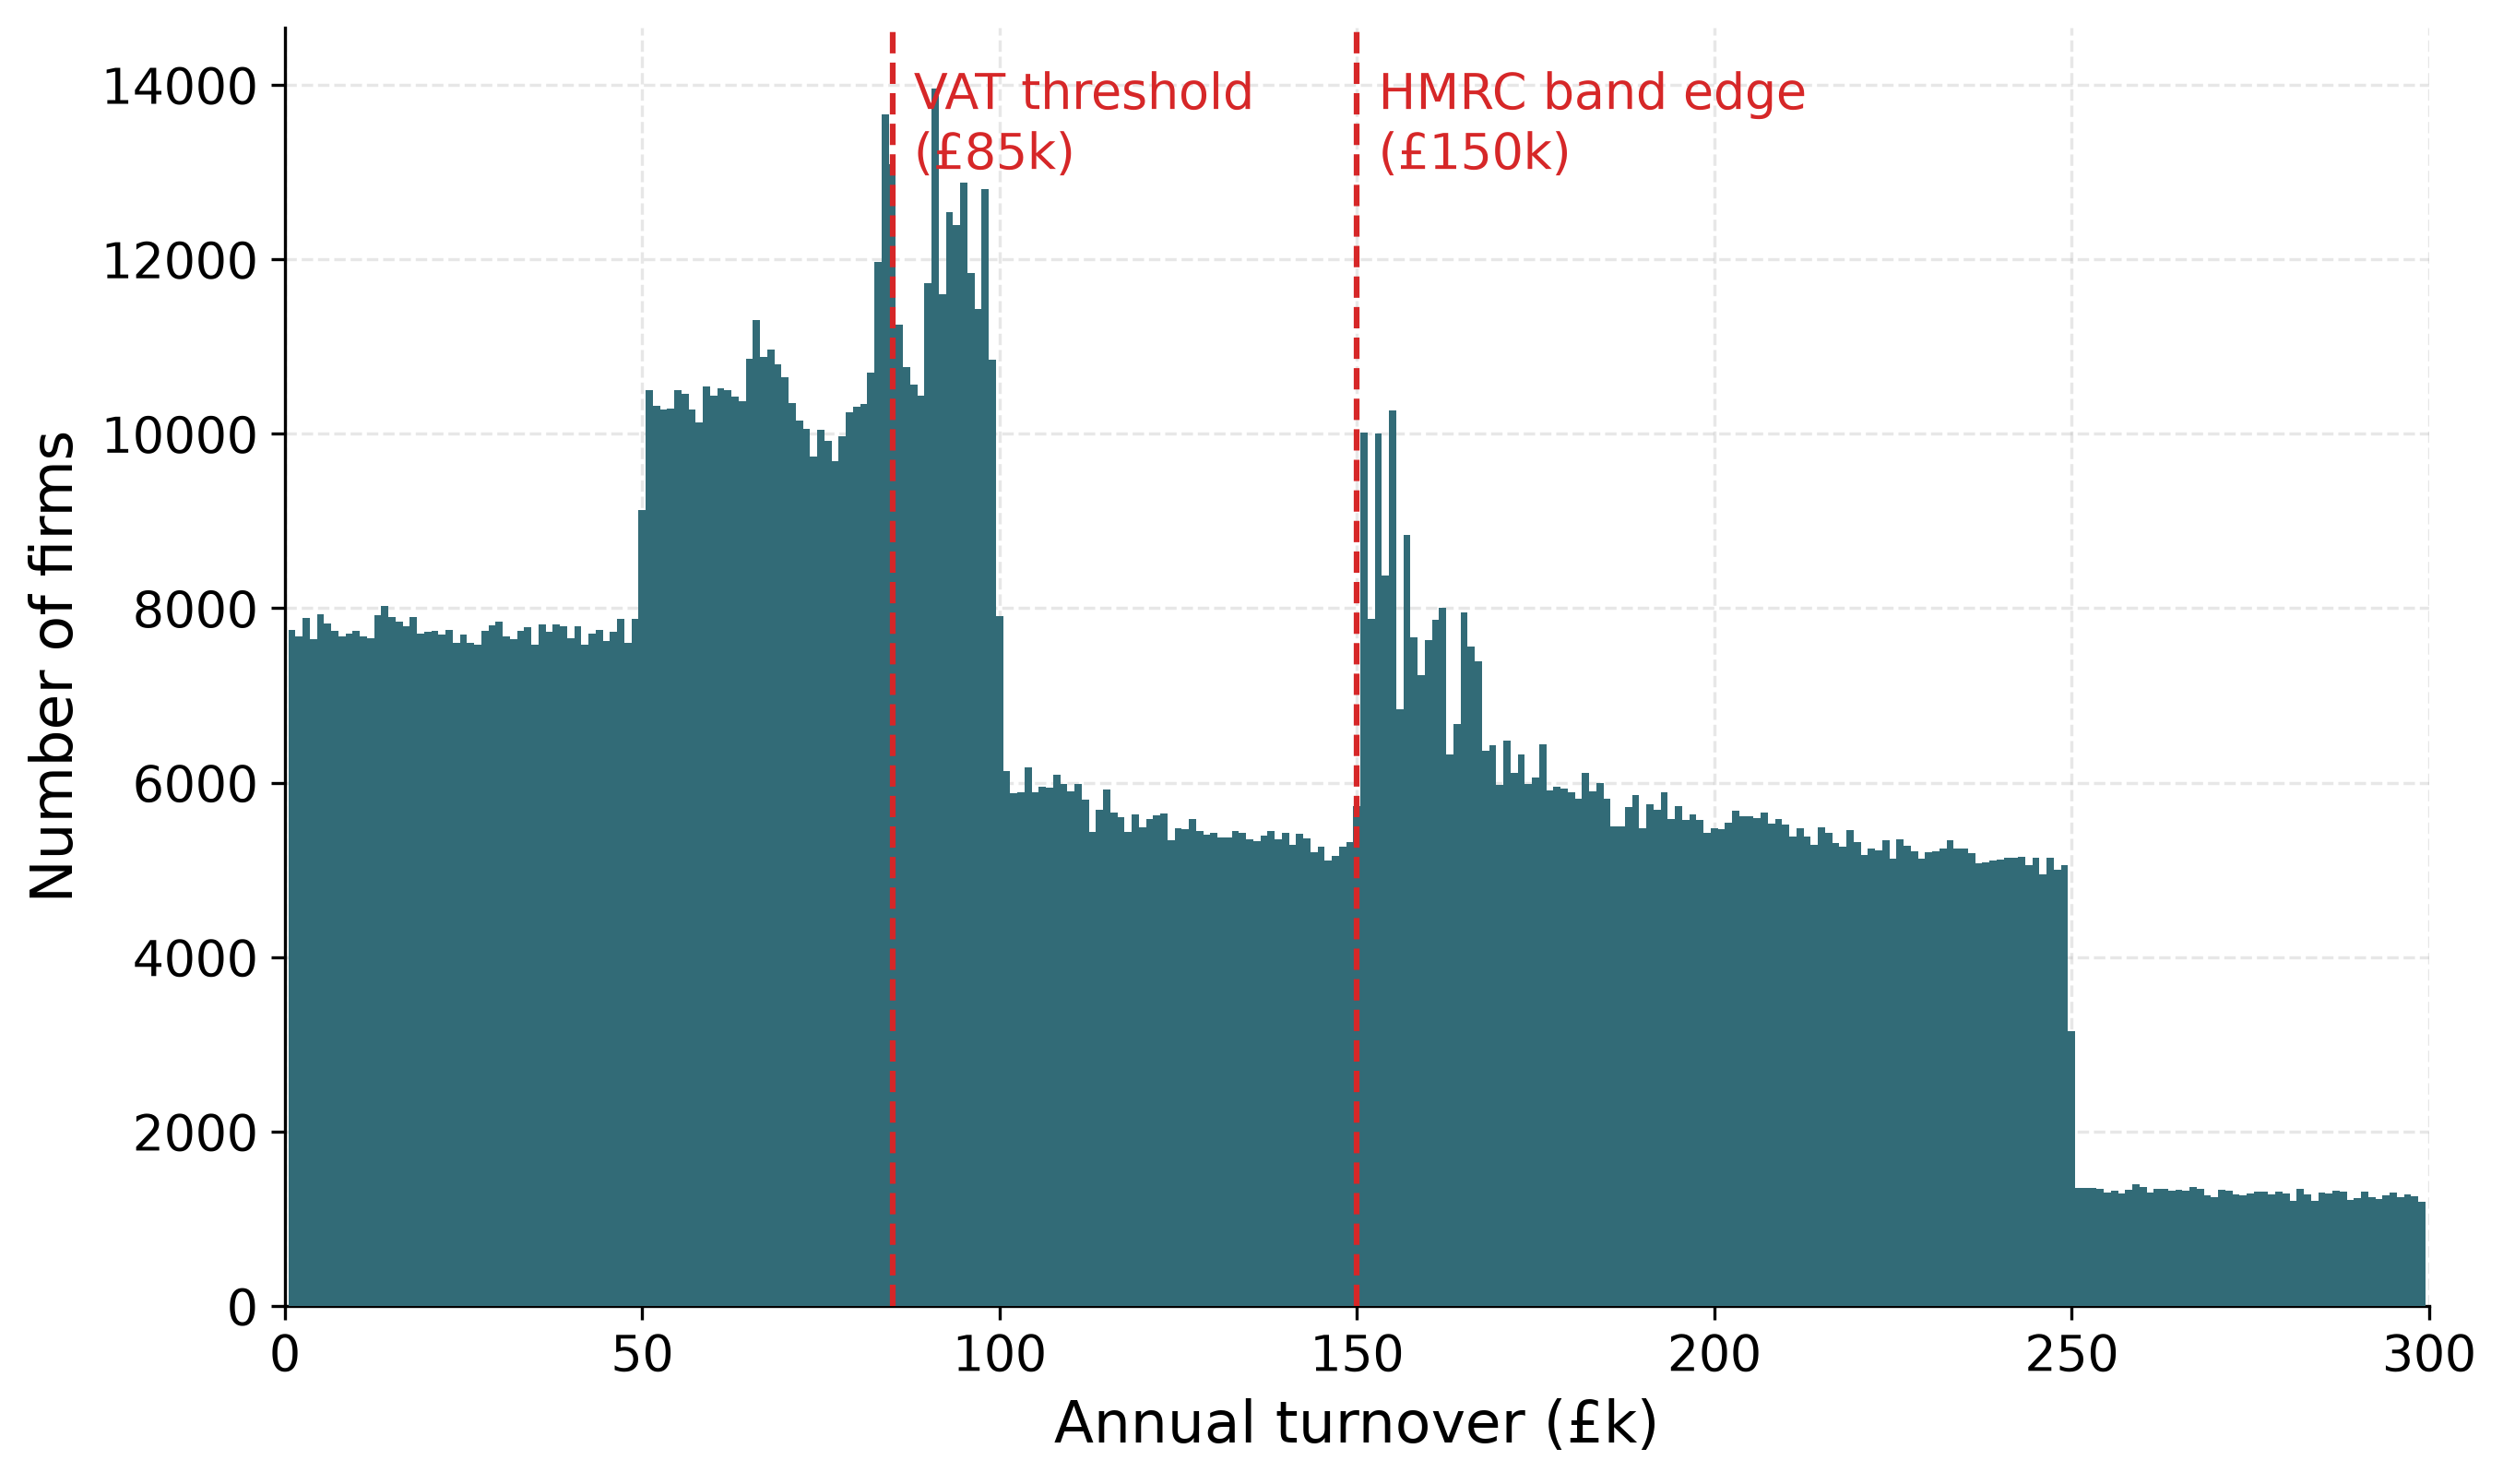
\includegraphics[width=0.74\textwidth]{figures/turnover_distribution_85k.png}
\caption{Synthetic firm turnover distribution (weighted firm counts,
\pounds1{,}000 bins), 2023--24. The near-threshold profile---rising into the
\pounds85{,}000 threshold and stepping down across it---is calibrated to the
OBR's published \pounds1{,}000-band counts and is therefore target-inherited,
not behavioural (Section~\ref{sec:bunching}). The seam at \pounds65{,}000
marks the edge of the published fine-band window; the \pounds150{,}000 step is
an HMRC calibration-band edge.}
\label{fig:turnover_dist}
\end{figure}
